\documentclass{article}
\usepackage{graphics}
\usepackage{nopageno}
\usepackage{txfonts}
\usepackage[usenames]{color}
\usepackage[T2A]{fontenc}
\usepackage[utf8]{inputenc}
%\usepackage{amsmath}

\begin{document}
\begin{center}
% GNUPLOT: LaTeX picture with Postscript
\begingroup
  \makeatletter
  \providecommand\color[2][]{%
    \GenericError{(gnuplot) \space\space\space\@spaces}{%
      Package color not loaded in conjunction with
      terminal option `colourtext'%
    }{See the gnuplot documentation for explanation.%
    }{Either use 'blacktext' in gnuplot or load the package
      color.sty in LaTeX.}%
    \renewcommand\color[2][]{}%
  }%
  \providecommand\includegraphics[2][]{%
    \GenericError{(gnuplot) \space\space\space\@spaces}{%
      Package graphicx or graphics not loaded%
    }{See the gnuplot documentation for explanation.%
    }{The gnuplot epslatex terminal needs graphicx.sty or graphics.sty.}%
    \renewcommand\includegraphics[2][]{}%
  }%
  \providecommand\rotatebox[2]{#2}%
  \@ifundefined{ifGPcolor}{%
    \newif\ifGPcolor
    \GPcolorfalse
  }{}%
  \@ifundefined{ifGPblacktext}{%
    \newif\ifGPblacktext
    \GPblacktexttrue
  }{}%
  % define a \g@addto@macro without @ in the name:
  \let\gplgaddtomacro\g@addto@macro
  % define empty templates for all commands taking text:
  \gdef\gplbacktext{}%
  \gdef\gplfronttext{}%
  \makeatother
  \ifGPblacktext
    % no textcolor at all
    \def\colorrgb#1{}%
    \def\colorgray#1{}%
  \else
    % gray or color?
    \ifGPcolor
      \def\colorrgb#1{\color[rgb]{#1}}%
      \def\colorgray#1{\color[gray]{#1}}%
      \expandafter\def\csname LTw\endcsname{\color{white}}%
      \expandafter\def\csname LTb\endcsname{\color{black}}%
      \expandafter\def\csname LTa\endcsname{\color{black}}%
      \expandafter\def\csname LT0\endcsname{\color[rgb]{1,0,0}}%
      \expandafter\def\csname LT1\endcsname{\color[rgb]{0,1,0}}%
      \expandafter\def\csname LT2\endcsname{\color[rgb]{0,0,1}}%
      \expandafter\def\csname LT3\endcsname{\color[rgb]{1,0,1}}%
      \expandafter\def\csname LT4\endcsname{\color[rgb]{0,1,1}}%
      \expandafter\def\csname LT5\endcsname{\color[rgb]{1,1,0}}%
      \expandafter\def\csname LT6\endcsname{\color[rgb]{0,0,0}}%
      \expandafter\def\csname LT7\endcsname{\color[rgb]{1,0.3,0}}%
      \expandafter\def\csname LT8\endcsname{\color[rgb]{0.5,0.5,0.5}}%
    \else
      % gray
      \def\colorrgb#1{\color{black}}%
      \def\colorgray#1{\color[gray]{#1}}%
      \expandafter\def\csname LTw\endcsname{\color{white}}%
      \expandafter\def\csname LTb\endcsname{\color{black}}%
      \expandafter\def\csname LTa\endcsname{\color{black}}%
      \expandafter\def\csname LT0\endcsname{\color{black}}%
      \expandafter\def\csname LT1\endcsname{\color{black}}%
      \expandafter\def\csname LT2\endcsname{\color{black}}%
      \expandafter\def\csname LT3\endcsname{\color{black}}%
      \expandafter\def\csname LT4\endcsname{\color{black}}%
      \expandafter\def\csname LT5\endcsname{\color{black}}%
      \expandafter\def\csname LT6\endcsname{\color{black}}%
      \expandafter\def\csname LT7\endcsname{\color{black}}%
      \expandafter\def\csname LT8\endcsname{\color{black}}%
    \fi
  \fi
  \setlength{\unitlength}{0.0500bp}%
  \begin{picture}(8502.00,5668.00)%
    \gplgaddtomacro\gplbacktext{%
      \csname LTb\endcsname%
      \put(946,704){\makebox(0,0)[r]{\strut{} 1}}%
      \csname LTb\endcsname%
      \put(946,1421){\makebox(0,0)[r]{\strut{} 1.2}}%
      \csname LTb\endcsname%
      \put(946,2138){\makebox(0,0)[r]{\strut{} 1.4}}%
      \csname LTb\endcsname%
      \put(946,2855){\makebox(0,0)[r]{\strut{} 1.6}}%
      \csname LTb\endcsname%
      \put(946,3573){\makebox(0,0)[r]{\strut{} 1.8}}%
      \csname LTb\endcsname%
      \put(946,4290){\makebox(0,0)[r]{\strut{} 2}}%
      \csname LTb\endcsname%
      \put(946,5007){\makebox(0,0)[r]{\strut{} 2.2}}%
      \csname LTb\endcsname%
      \put(1078,484){\makebox(0,0){\strut{} 1}}%
      \csname LTb\endcsname%
      \put(2835,484){\makebox(0,0){\strut{} 2}}%
      \csname LTb\endcsname%
      \put(4592,484){\makebox(0,0){\strut{} 3}}%
      \csname LTb\endcsname%
      \put(6348,484){\makebox(0,0){\strut{} 4}}%
      \csname LTb\endcsname%
      \put(8105,484){\makebox(0,0){\strut{} 5}}%
      \put(176,2855){\rotatebox{-270}{\makebox(0,0){\strut{}efficiency ratio $R=E_{p}/E_{56}$}}}%
      \put(4591,154){\makebox(0,0){\strut{}pipeline stages}}%
      \put(4591,5337){\makebox(0,0){\strut{}Figure 3 (DUMMY)}}%
    }%
    \gplgaddtomacro\gplfronttext{%
      \csname LTb\endcsname%
      \put(4874,4834){\makebox(0,0)[l]{\strut{}$p=112$ cores, SSH TM}}%
      \csname LTb\endcsname%
      \put(4874,4614){\makebox(0,0)[l]{\strut{}$p=224$ cores, SSH TM}}%
      \csname LTb\endcsname%
      \put(4874,4394){\makebox(0,0)[l]{\strut{}$p=112$ cores, Shared TM}}%
      \csname LTb\endcsname%
      \put(4874,4174){\makebox(0,0)[l]{\strut{}$p=224$ cores, Shared TM}}%
    }%
    \gplbacktext
    \put(0,0){\includegraphics{fig}}%
    \gplfronttext
  \end{picture}%
\endgroup

\end{center}
Ratios of the mapping time~$T_{mapping}$ to the communication costs~$T_{comm}$ for HPC2 and Hadoop clusters for Dataset IV as a function of reciprocal cluster size $1/N$. Two HPC scenarios are shown as ``HPC SLURM'' and ``HPC random'', which correspond to standard SLURM behaviour and a modified one, where nodes are being allocated from random racks.
%One  can see the differences in the Hadoop and HPC communication patterns: for Hadoop the ratio is almost constant, while for HPC cluster there are two defined regions.
%The first one resembles to that of Hadoop, and corresponds to the case then the communication in the cluster is not a bottleneck. 
%The second one shows the regime corresponding to the case of saturation of the network, resulting in traffic jams: data distibution time~$T_{comm}$ stops to scale 
%linearly to the reciprocal cluster size, and becomes more of less a constant, while the mapping time continues to satisfy~$T_{mapping}\propto 1/N$.
Linear fit  done with the least-squares method.
\end{document}
